\documentclass{report}

% Ćirilica: kodiranje fonta i jezik (srpski, ćirilica)
\usepackage[T2A]{fontenc}
\usepackage[utf8]{inputenc}
\usepackage[serbianc]{babel}

% Veličina strane i margine
\usepackage[a4paper,top=2cm,bottom=2cm,left=3cm,right=3cm,marginparwidth=1.75cm]{geometry}

% Korisni paketi
\usepackage{amsmath}
\usepackage{graphicx}
\usepackage{float}

\usepackage{subcaption}
\usepackage{enumitem}

\usepackage{booktabs}
\usepackage{tcolorbox}
\tcbuselibrary{breakable}
\usepackage[colorlinks=true, allcolors=blue]{hyperref}

% Цртежи (TikZ)
\usepackage{tikz}
\usetikzlibrary{arrows.meta, calc, decorations.markings, babel}

% TikZ стилови који се понављају на цртежима
\tikzset{
    naboj/.style={circle, draw, thick, minimum size=6mm, inner sep=0pt, font=\small},
    jezgro/.style={circle, draw, thick, fill=gray!15, minimum size=7mm, inner sep=0pt, font=\small},
    elektron/.style={circle, draw, fill=cyan!30, inner sep=0pt, minimum size=5pt},
    supljina/.style={circle, draw, thick, minimum size=5mm, inner sep=0pt, font=\small},
    sredstrelica/.style={postaction={decorate}, decoration={markings, mark=at position 0.55 with {\arrow{Stealth}}}},
    % --- графици наизменичних величина ---
    pomocna/.style={dashed, gray!70, thin},
    mreza/.style={gray!25, very thin},
    kriva/.style={very thick, red!75!black},
    % --- проводник у пресеку: празан, тачка (ка нама), крстић (од нас) ---
    provodnik/.style={circle, draw, thick, fill=white, minimum size=8pt, inner sep=0pt},
    provodnikT/.style={provodnik, path picture={\fill[black] (path picture bounding box.center) circle (1.1pt);}},
    provodnikK/.style={provodnik, path picture={
        \draw (path picture bounding box.south west) -- (path picture bounding box.north east)
              (path picture bounding box.north west) -- (path picture bounding box.south east);}},
    oznaka/.style={fill=white, inner sep=1pt, font=\small},
}

% Оквир за решене примере
\newtcolorbox[auto counter]{primer}{breakable,
    colback=white, colframe=black!55, colbacktitle=black!55, coltitle=white,
    fonttitle=\bfseries\small, title={Пример~\thetcbcounter},
    boxrule=0.5pt, arc=1.5pt, left=6pt, right=6pt, top=3pt, bottom=3pt,
    before skip=8pt, after skip=10pt}

% Оквир за кључне формуле
\newtcolorbox{kljucno}{colback=blue!4, colframe=blue!45!black,
    boxrule=0.5pt, arc=1.5pt, left=8pt, right=8pt, top=4pt, bottom=4pt}

% Слика: ако фајл још не постоји, црта се празан оквир са именом фајла
%   #1 -- ширина (део ширине текста), #2 -- име фајла у фолдеру slike, #3 -- натпис

\title{Аутоелектронски системи 2 - Jetronic системи убризгавања - наставак}
\author{Саобраћајно техничка школа, Београд, Земун}

\begin{document}
\maketitle

\tableofcontents
\newpage

%##################################################################
\chapter{Mono-Jetronic}
%##################################################################

За разлику од KE-Jetronic и L-Jetronic система, овај систем има \textbf{централно}
убризгавање. Централни колектор равномерно распоређује гориво према појединим
цилиндрима и његова највећа примена је у четвороцилиндричним моторима.

Потребне информације о раду мотора се прикупљају помоћу сензора и даље се обрађују
у ЕУЈ (електронска управљачка јединица). На основу свих информација
израђују се управљачки сигнали за \textbf{вентил убризгавања, корачни мотор за
регулацију празног хода и вентил утрошка бензинских испарења}.

\section{Принцип убризгавања}

Код KE и L-Jetronic система свака бризгаљка убризгава гориво испред усисног
вентила свог цилиндра (убризгавање у више тачака, MPI). Mono-Jetronic има само
\textbf{једну бризгаљку}, смештену у централној јединици изнад пригушног
лептира, на самом почетку усисне цеви (убризгавање у једној тачки, SPI).
Бризгаљка је електромагнетни вентил, а количину горива одређује управљачка
јединица дужином импулса, тј. временом за које држи бризгаљку отвореном.
Гориво се затим, заједно са ваздухом, кроз усисни колектор разводи до свих
цилиндара.

\begin{figure}[H]
    \centering
    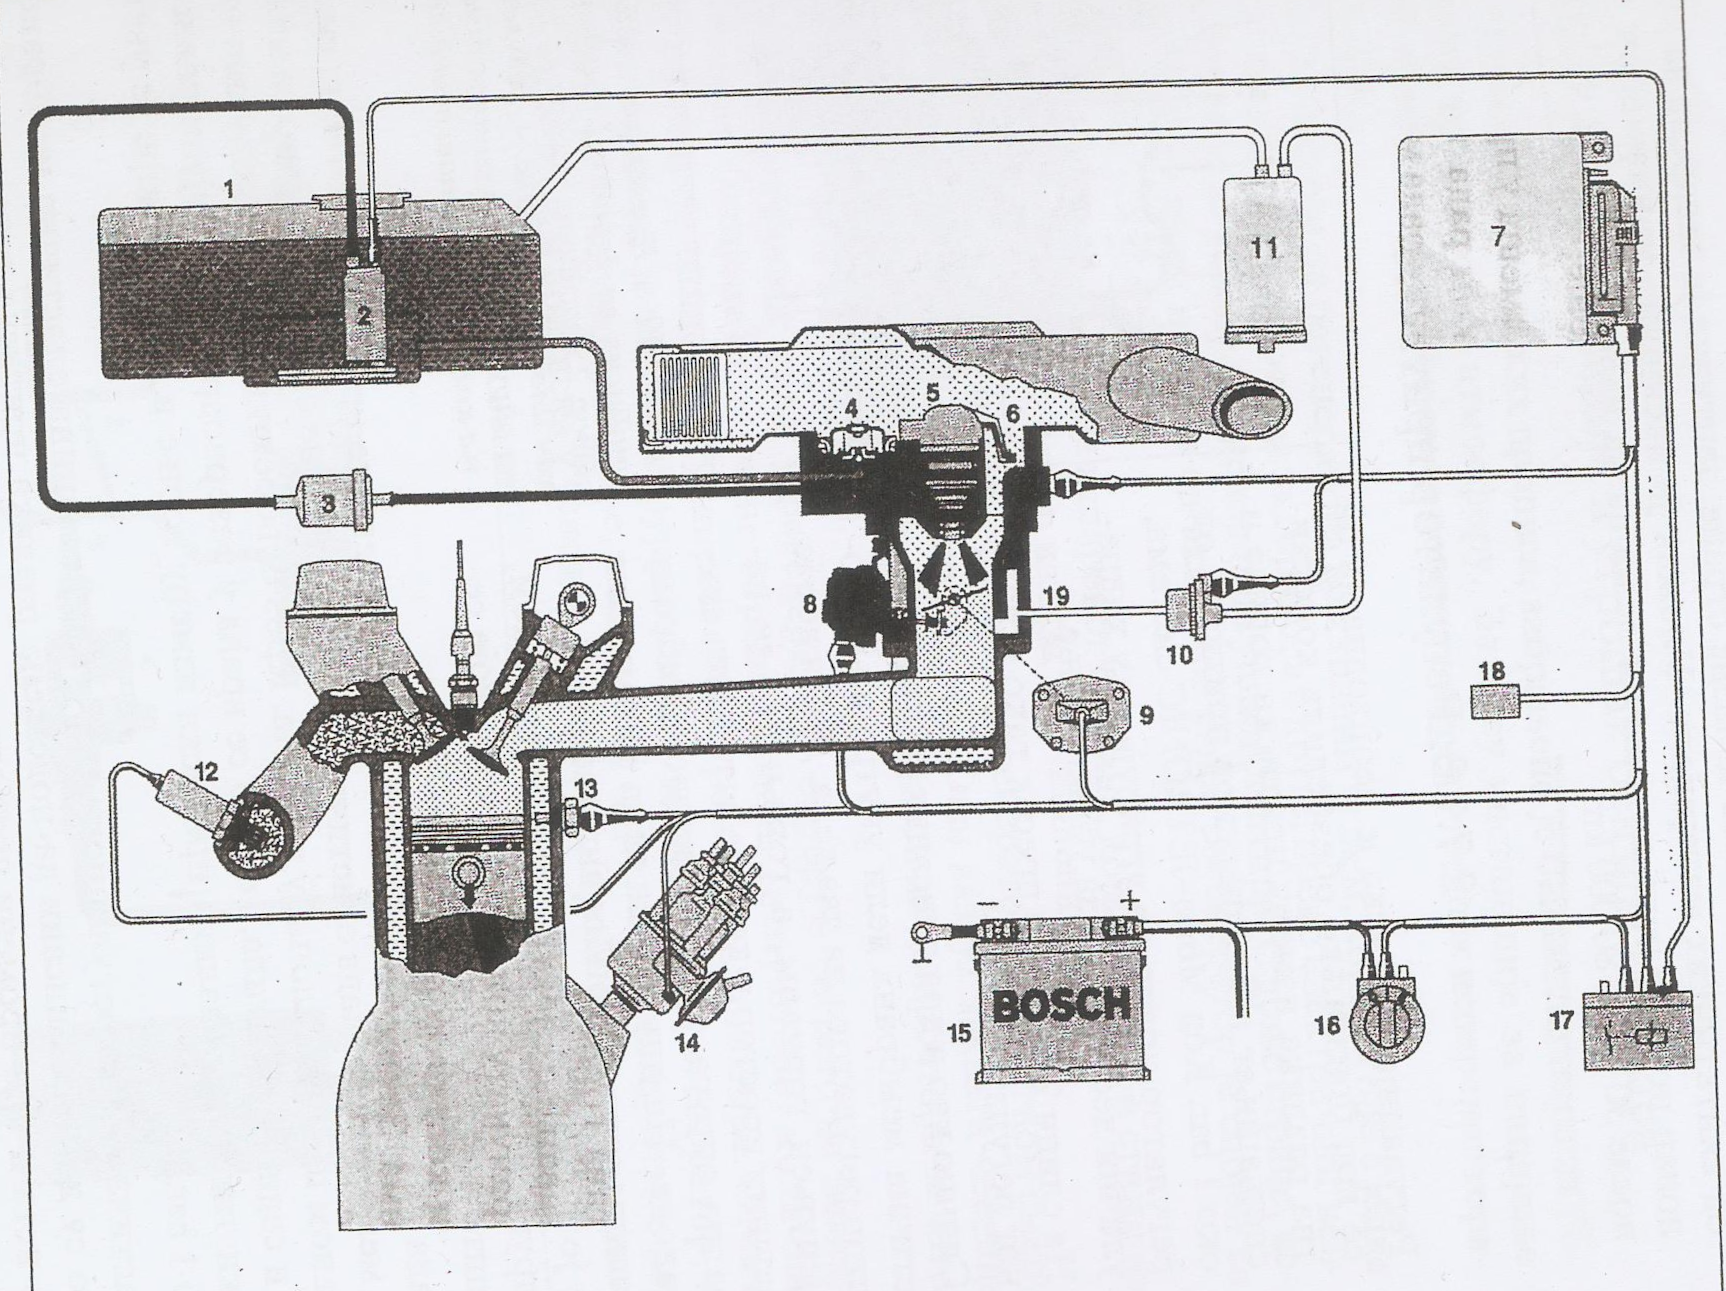
\includegraphics[width=0.7\textwidth]{slike/Mono.png}
    \caption{Основна шема Mono-Jetronic система убризгавања}
    \label{fig:mono-sema}
\end{figure}

\begin{kljucno}

      \begin{enumerate}[noitemsep]
    \item[1.] Резервоар за гориво
    \item[2.] Електрична пумпа
    \item[3.] Филтер за гориво
    \item[4.] Регулатор притиска
    \item[5.] Електромагнетна бризгаљка
    \item[6.] Сензор температуре усисаног ваздуха
    \item[7.] Електронска управљачка јединица
    \item[8.] Корачни (степ) мотор
    \item[9.] Потенциометар пригушног лептира
    \item[10.] Вентил за регенерисано гориво (EVAP)
    \item[11.] Регенератор са активним угљем
    \item[12.] ЛАМБДА сонда
    \item[13.] Сензор температуре мотора
    \item[14.] Разводник паљења
    \item[15.] Акумулатор
    \item[16.] Контакт-кључ
    \item[17.] Електронски релеј
    \item[18.] Прикључак за дијагностику
    \item[19.] Уређај за убризгавање (централна јединица)
\end{enumerate}
      
\end{kljucno}

\section{Шта решава и по коју цену}

KE и L-Jetronic су прецизни, али скупи системи: имају по једну бризгаљку за сваки
цилиндар, мерач протока ваздуха, систем под високим притиском и много
механичких или електронских делова. За мале и јефтине аутомобиле то је било
прескупо, а карбуратор више није могао да испуни строге прописе о издувним
гасовима, нарочито уз катализатор, који тражи смешу са $\lambda \approx 1$.

Mono-Jetronic је настао као \textbf{јефтина замена за карбуратор}, која задржава
главне предности електронског убризгавања:

\begin{itemize}[noitemsep]
    \item \textbf{једна бризгаљка} уместо четири, и централна јединица која се
          уграђује на место карбуратора, па се мотор мало мења,
    \item \textbf{низак притисак горива} (око 1~bar), па су пумпа, водови и
          регулатор једноставнији и јефтинији,
    \item \textbf{нема мерача протока ваздуха}: количина ваздуха се израчунава
          посредно, из угла пригушног лептира и броја обртаја,
    \item електронска регулација са ЛАМБДА сондом, па систем ради са
          трокомпонентним катализатором и испуњава прописе.
\end{itemize}

\textbf{Цена} тих уштеда је мања прецизност. Гориво путује од бризгаљке до
цилиндара кроз цео усисни колектор, па:

\begin{itemize}[noitemsep]
    \item део горива се таложи на зидовима колектора као филм, па смеша није
          иста у свим цилиндрима, нарочито код хладног мотора,
    \item при наглим променама оптерећења смеша касни за потребама мотора, па
          су потребне посебне корекције,
    \item посредно мерење ваздуха мање је тачно од мерача протока, па систем
          мора стално да се прилагођава (адаптација),
    \item снага и економичност мотора су нешто мањи него са убризгавањем у
          више тачака.
\end{itemize}

Због тога се Mono-Jetronic највише користио код мањих четвороцилиндричних
мотора, где су ниска цена и испуњење еколошких прописа били важнији од највеће
снаге.

\section{Шта је додато или промењено у односу на KE и L-Jetronic}

\begin{table}[H]
    \centering
    \small
    \renewcommand{\arraystretch}{1.3}
    \begin{tabular}{p{4.2cm} p{4.6cm} p{4.6cm}}
        \toprule
                                & \textbf{KE / L-Jetronic}               & \textbf{Mono-Jetronic} \\
        \midrule
        бризгаљке               & по једна за сваки цилиндар              & једна, централна \\
        место убризгавања       & испред усисних вентила                  & изнад пригушног лептира \\
        притисак горива         & око 2,5--5~bar                          & око 1~bar \\
        мерење ваздуха          & мерна плоча / заклопка                  & нема мерача, рачуна се из $\alpha$ и $n$ \\
        пригушни лептир         & прекидач лептира                        & потенциометар са две отпорне траке \\
        празан ход              & биметални вентил / регулатор празног хода & корачни мотор помера лептир \\
        хладан старт            & бризгаљка за хладан старт               & продужење импулса главне бризгаљке \\
        пумпа                   & у водовима (in-line)                    & у резервоару (in-tank) \\
        \bottomrule
    \end{tabular}
    \caption{Најважније разлике у односу на KE и L-Jetronic}
\end{table}

%##################################################################
\chapter{Компоненте Mono-Jetronic система}
%##################################################################

\section{Преглед компоненти}

Систем се може поделити на три групе:

\begin{kljucno}
\begin{itemize}[noitemsep]
    \item \textbf{инсталација за напајање горивом}: електрична пумпа, филтер,
          регулатор притиска, регенератор са активним угљем и EVAP вентил,
    \item \textbf{уређај за убризгавање}: централна јединица са бризгаљком,
          регулатором притиска, пригушним лептиром, потенциометром, корачним
          мотором и сензором температуре ваздуха,
    \item \textbf{електронски део}: управљачка јединица, сензори (ЛАМБДА
          сонда, температура мотора, број обртаја) и релеји.
\end{itemize}
\end{kljucno}

\section{Електрична пумпа за гориво}

Пумпа се поставља \textbf{директно у резервоар} (in-tank систем). У посебном
држачу у резервоару налазе се пумпа и филтер на усисној страни, а држач има
прикључке за гориво и електрично напајање. Код ранијих система
пумпа је била у водовима, између резервоара и филтера (in-line систем).
Предност пумпе у резервоару је што гориво хлади пумпу и пригушује њену буку.

Користи се \textbf{двостепена пумпа} са мотором једносмерне
струје у истом кућишту. На потисној страни налазе се електрични прикључак и
неповратни вентил, који не дозвољава повратак горива после искључења пумпе и
одржава притисак у инсталацији. Тако се спречава стварање мехурића паре у
загрејаном гориву.

Оба степена пумпе су радијална и налазе се на истом радном колу.
Први степен, мањег пречника, усисава гориво и потискује га ка спољном отвору
другог степена, који повећава притисак и потискује гориво у унутрашњост
мотора пумпе. На усисном делу је мали мембрански вентил, који избацује
мехуриће ваздуха и паре настале током рада пумпе. Пумпа има задовољавајући
капацитет и при високим температурама и ради врло тихо.

\begin{figure}[H]
    \centering
    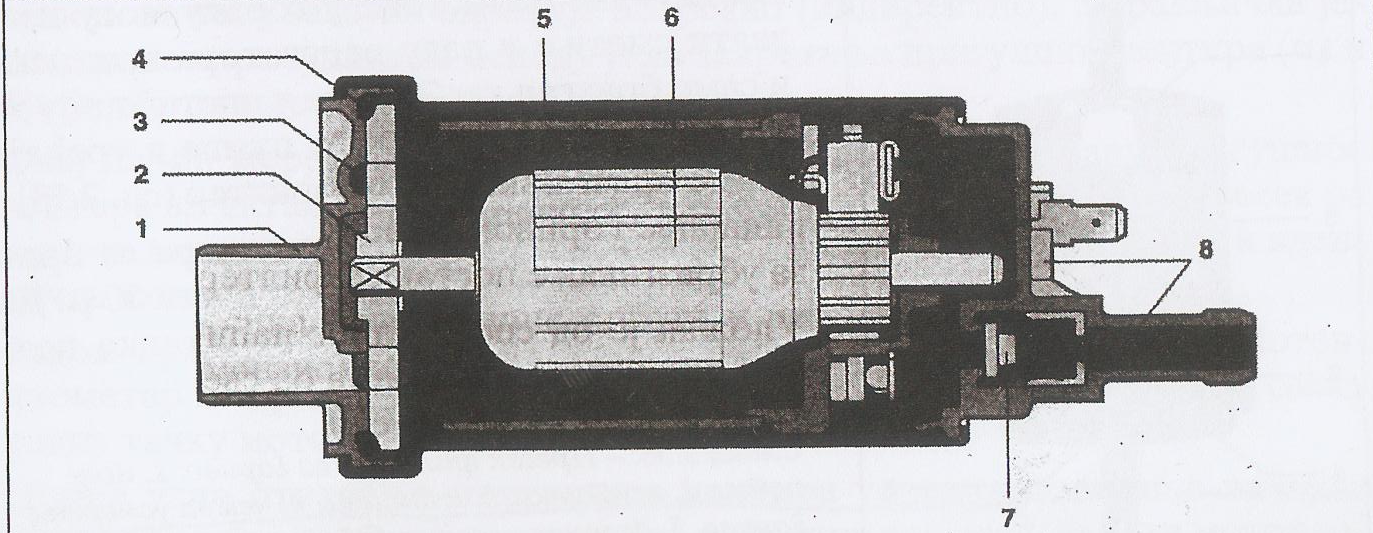
\includegraphics[width=0.4\textwidth]{slike/1.png}
    \caption{Електрична пумпа за гориво}
    \label{fig:mono-sema}
\end{figure}

\section{Филтер за гориво}

Нечистоће у гориву могу изазвати сметње у раду регулатора притиска и саме
бризгаљке. Зато се филтер уграђује у инсталацију између пумпе и уређаја за
убризгавање. Уложак је од специјалног папира са порама од око
10~$\mu$m. Кућиште је, због строгих захтева за заптивеност, заварено, а
уложак се ослања на потпорну плочу. Филтер се мења према упутству
произвођача, обично после 30\,000 до 80\,000~km.

\section{Регулатор притиска}

Регулатор одржава \textbf{сталну разлику притиска} између горива и околине
(око 1~bar), да би бризгаљка при истој дужини импулса увек убризгала исту
количину горива. Код Mono-Jetronic система уграђује се у хидраулични део
уређаја за убризгавање.

Еластична мембрана дели регулатор на две коморе. Доња комора је испуњена
горивом, а у горњој је регулациона опруга, која потискује мембрану надоле.
На мембрани је плочица вентила. Када притисак горива порасте изнад подешене
вредности, сила горива савлада опругу, мембрана се подигне и отвори вентил,
па вишак горива отиче у повратни вод ка резервоару. Тако се притисак одржава
сталним без обзира на количину потрошеног горива. Када се мотор угаси,
вентил се затвори, па у инсталацији још неко време остаје притисак, што
спречава стварање мехурића и олакшава поновно паљење топлог мотора.

\section{Регенерација и утрошак бензинских пара}

Прописи забрањују испуштање бензинских пара из резервоара у атмосферу. Зато
су инсталације опремљене уређајем за регенерацију и утрошак тих пара. Уређај чине \textbf{регенератор са активним угљем} и електрични
\textbf{EVAP вентил}. Регенератор је са једне стране спојен са резервоаром, а
са друге, преко EVAP вентила, са усисном цеви испод пригушног лептира. Доња
страна регенератора има отвор ка атмосфери.

Активни угаљ упија честице бензинских пара из резервоара. Када EVAP вентил
отвори пролаз, потпритисак у усисној цеви повлачи свеж ваздух кроз
регенератор у супротном смеру. Ваздух понесе упијено гориво и одводи га у
цилиндре, где сагори, а угаљ се тиме чисти за ново упијање.

\begin{figure}[H]
    \centering
    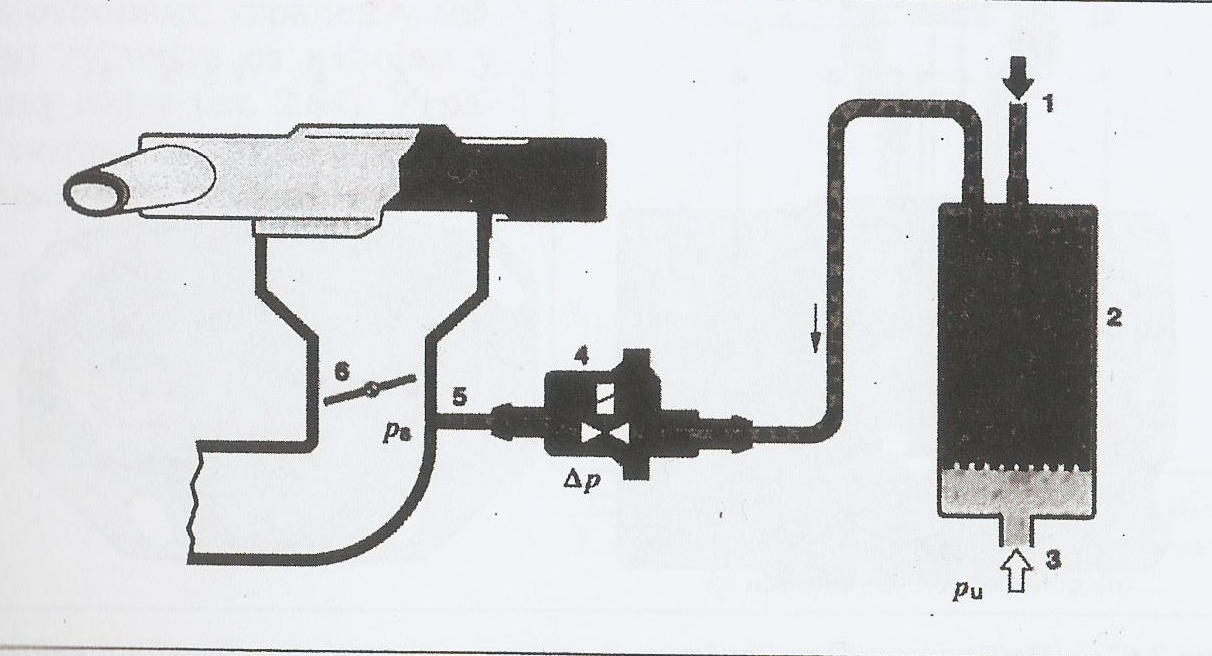
\includegraphics[width=0.4\textwidth]{slike/2.png}
    \caption{Регенерација и утрошак бензинских пара}
    \label{fig:mono-sema}
\end{figure}

Количина горива из регенератора зависи од разлике притисака, која је највећа
у празном ходу, када је регенератор пун горива. Тада би неконтролисано
доведено гориво пореметило смешу, а при пуном оптерећењу је обрнуто: разлика
притисака је мала, па је и проток мали. Проблем решава EVAP вентил, чијим
отварањем управља електронска управљачка јединица, према програму и тренутном
режиму рада мотора.

\section{Електрични (EVAP) вентил регенератора}

Уређај за регенерацију упија испарено гориво из резервоара помоћу активног
угља. Када се угаљ засити, гориво се, зависно од режима рада мотора, струјањем
свежег ваздуха враћа у усисну цев. Циљ је да се гориво враћа само у тренуцима
када то не ремети рад мотора. Количина горива из регенератора може да износи
и 20\,\% од укупне количине у радној смеши, па се у фази пражњења
регенератора адаптација смеше не врши.

\textbf{EVAP вентил} конструисан је тако да пропушта количину
ваздуха која није сразмерна разлици притисака на улазу и излазу. Када је та
разлика највећа (празан ход), пропусна моћ вентила је најмања, јер режим празног
хода не сме да се ремети. При пуном оптерећењу, када је разлика најмања,
пропусна моћ је највећа, па мотор добија највише горива из регенератора.

Вентил је електромагнетни са еластичном котвом, која се затвара у смеру
кретања ваздуха. Без струје опруга (3) држи котву (5) на седишту и пролаз је
затворен. Када јединица пусти импулс, магнет привуче котву, вентил се отвори
и ваздух са горивом из регенератора отиче у усисну цев. У свим режимима
радом вентила управља јединица, импулсима одређеног трајања и учестаности.

\section{Уређај за убризгавање}

Уређај за убризгавање је најважнији део система и поставља се на почетак
усисне цеви, на место где је раније био карбуратор. Уређај има два дела:

\begin{itemize}[noitemsep]
    \item \textbf{хидраулични део} (горњи): бризгаљка, регулатор притиска,
          сензор температуре усисаног ваздуха и канали за довод и одвод
          горива,
    \item \textbf{доњи део}: пригушни лептир са потенциометром и корачни мотор
          за подешавање почетног положаја лептира у празном ходу.
\end{itemize}

\begin{figure}[H]
    \centering
    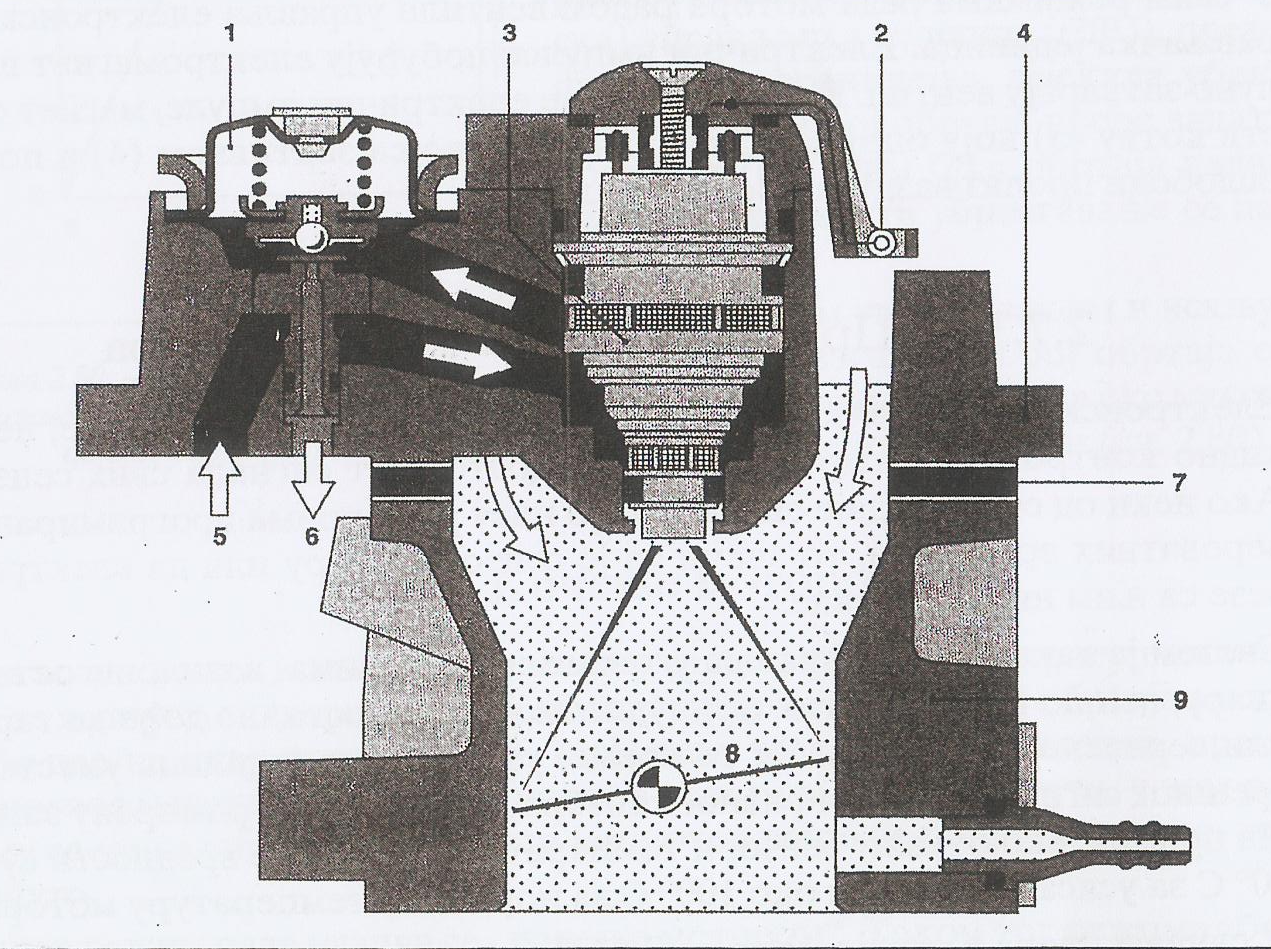
\includegraphics[width=0.5\textwidth]{slike/21.png}
    \caption{Бризгаљка}
    \label{fig:mono-sema}
\end{figure}

Гориво кроз доњи канал улази, а кроз горњи, преко регулатора притиска, вишак
горива се враћа у резервоар. Посебан распоред канала омогућава да гориво
стално струји око бризгаљке и хлади је, па се мехурићи паре не задржавају у
загрејаном гориву.

\begin{figure}[H]
    \centering
    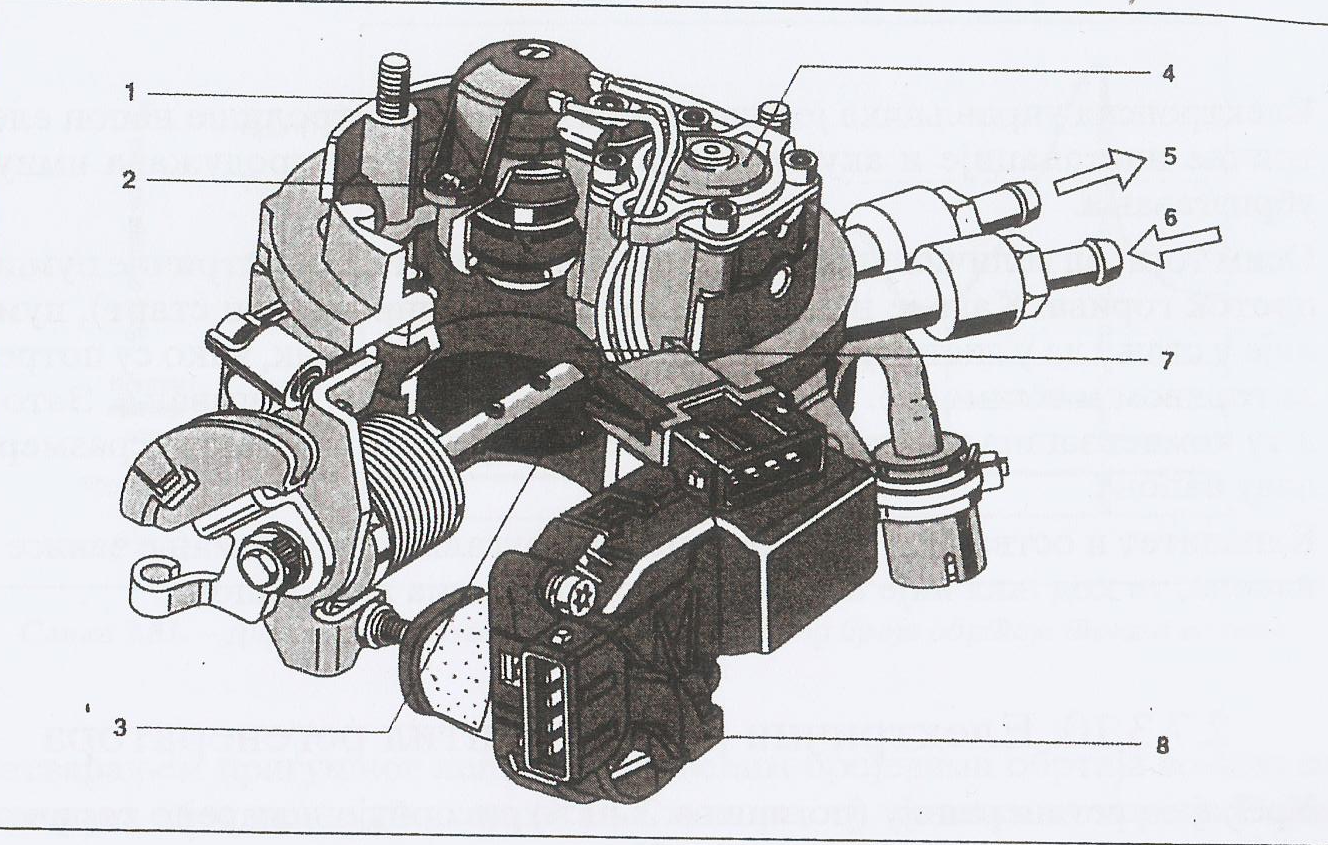
\includegraphics[width=0.5\textwidth]{slike/22.png}
    \caption{Систем убризгавања}
    \label{fig:mono-sema}
\end{figure}

\section{Бризгаљка - вентил убризгавања}

Бризгаљка се налази у горњем делу уређаја, у посебно обликованом
држачу, у средини ваздушне струје. Тако млаз горива пада тачно у простор
између кућишта и пригушног лептира, где ваздух струји највећом брзином, па се
гориво добро меша са ваздухом.

Бризгаљка се састоји од кућишта, у коме је намотај електромагнета, и
вентилског дела са иглом и котвом. У мировању опруга потискује иглу на
седиште и вентил је затворен. Када управљачка јединица пусти струју кроз
намотај, магнет привуче котву и подигне иглу за око 0,06~mm, па гориво кроз
посебно обликовану млазницу излази у облику купе. Пошто је притисак сталан,
количина убризганог горива зависи само од времена отварања.

Покретни део бризгаљке има врло малу масу, па се отвара и затвара веома
брзо. Најмање време отварања је око 1~ms, па се количина горива може тачно
дозирати и при врло малим потребама мотора.

\section{Корачни мотор пригушног лептира}

Корачни (степ) мотор подешава почетни положај пригушног лептира
у празном ходу. Састоји се од малог електромотора једносмерне струје, чији
пужасти пренос, преко зупчаника, аксијално помера малу осовину. Осовина се
наслања на полугу пригушног лептира и мења му почетни положај. На врху
осовине налази се прекидач празног хода, који се затвара када полуга лептира
належе на осовину.

\begin{figure}[H]
    \centering
    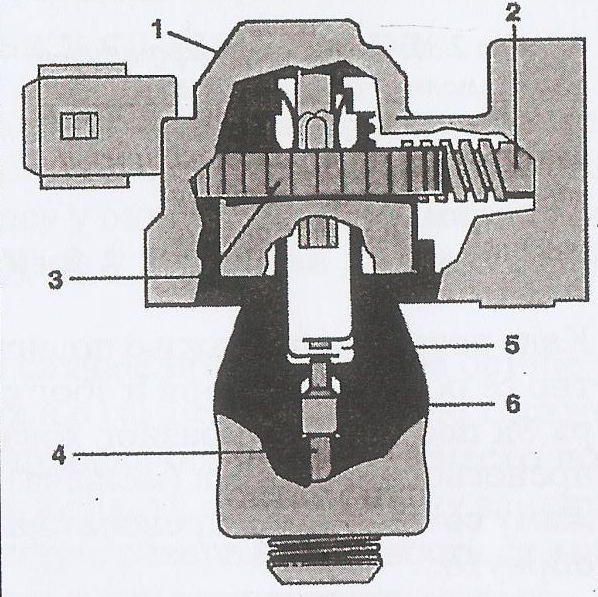
\includegraphics[width=0.5\textwidth]{slike/18.png}
    \caption{Корачни мотор}
    \label{fig:mono-sema}
\end{figure}

%##################################################################
\chapter{Сензори}
%##################################################################

Помоћу сензора прикупљају се сви важни подаци о раду мотора. Они се у облику
електричних сигнала доводе до управљачке јединице, где се аналогни сигнали
претварају у дигиталне, а затим обрађују у микропроцесору. На основу
резултата јединица управља извршним органима.

\section{Усисана количина ваздуха}

Пре Mono-Jetronic система сви системи су количину усисаног ваздуха мерили
посебним мерачем (протокомером). Код Mono-Jetronic система она се одређује
\textbf{посредно}: управљачка јединица је израчунава из \textbf{угла
отварања пригушног лептира ($\alpha$)} и \textbf{броја обртаја мотора ($n$)}.

Оваква метода захтева прецизну израду лептира и кућишта. Пресек између лептира
и кућишта за исти угао мора бити исти код сваког уређаја. Положајем лептира
управља возач преко педале гаса, а потенциометар региструје угао за сваки
положај.

Количина усисаног ваздуха зависи од угла и броја обртаја. За дати мотор
зависност се одреди мерењем на испитном столу и сними у дијаграм.
На вертикалној оси је релативно пуњење ваздухом, на хоризонталној број
обртаја, а свака крива одговара једном углу лептира. Уз претпоставку сталне
густине ваздуха, из угла $\alpha$ и броја обртаја $n$ може се одредити
количина ваздуха, а тиме и време убризгавања.

\begin{figure}[H]
    \centering
    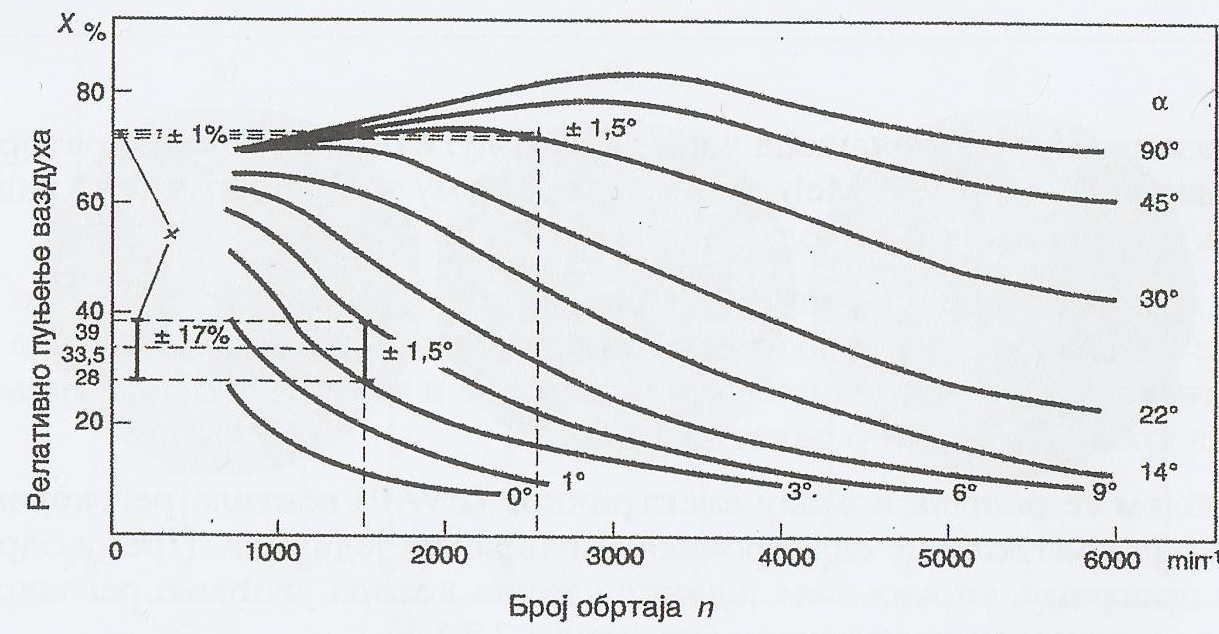
\includegraphics[width=0.5\textwidth]{slike/3.png}
    \caption{График одређивања}
    \label{fig:mono-sema}
\end{figure}

Из дијаграма се види да количина ваздуха није сразмерна углу лептира. При
малом броју обртаја ($n = 1000$--$2000$~min$^{-1}$) и малим угловима
($\alpha = 1$--$10^\circ$), промена угла од само $1{,}5^\circ$ мења пуњење за
око 17\,\%, а у подручју средњих обртаја и углова иста промена угла мења га
за свега 1,5\,\%. Зато је мерење угла веома важно, нарочито при малим
оптерећењима и у празном ходу.

Пошто густина ваздуха зависи и од температуре и атмосферског притиска,
управљачка јединица подешава време убризгавања и према температури ваздуха,
а остале корекције врши на основу сигнала ЛАМБДА сонде. Те корекције се памте
и користе и после гашења мотора (адаптивна корекција).

\section{Угао пригушног лептира}

На основу угла лептира управљачка јединица израчунава положај и брзину кретања
лептира. Из положаја се одређује количина ваздуха, а из брзине померања
компензација смеше у прелазним режимима.

\textbf{Потенциометар пригушног лептира} има клизач чврсто
спојен са осовином лептира. На кућишту од изолационог материјала налазе се
отпорне и проводне траке, а напаја се стабилизованим напоном од 5~V. Прва
отпорна трака мери угао од 0 до $24^\circ$, а друга од 18 до $90^\circ$, па је
мерење тачно и за мале и за велике углове. Јединица добија аналоган сигнал,
који се претвара у дигитални. На тачност мерења не утичу ни старење, ни
хабање, ни промена температуре, јер јединица посматра само промену напона.

\begin{figure}[H]
    \centering
    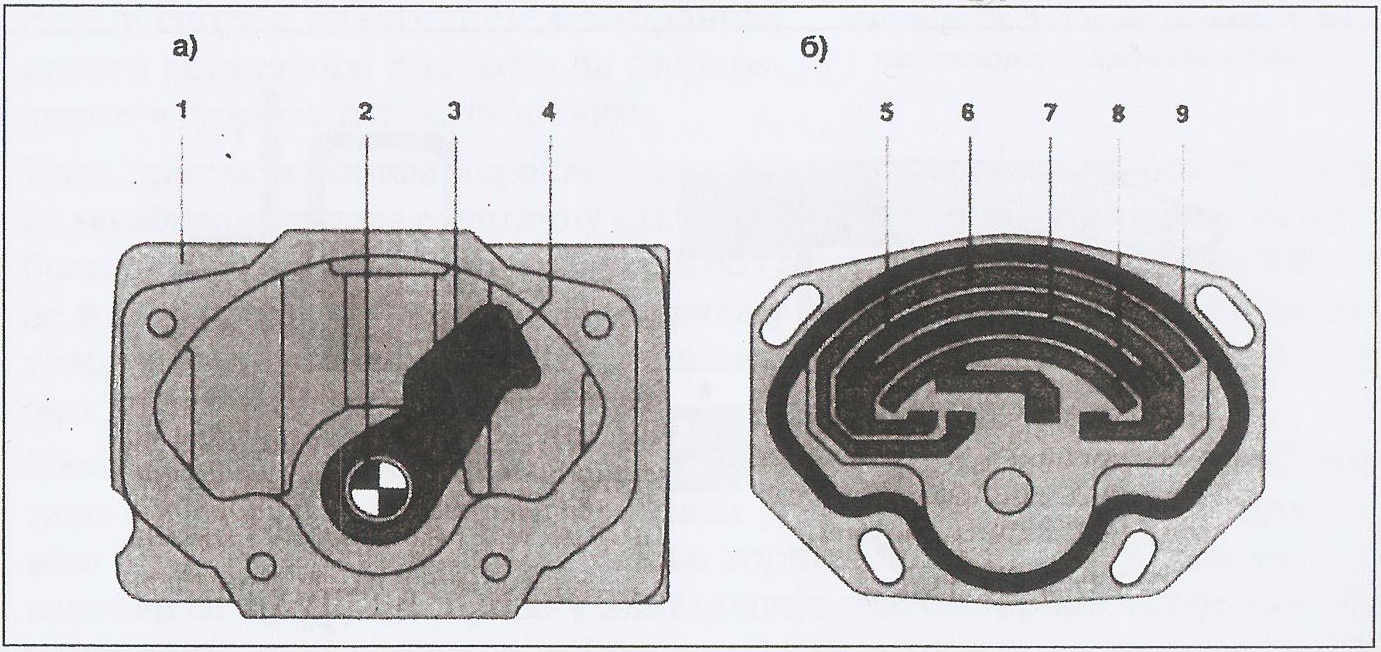
\includegraphics[width=0.5\textwidth]{slike/4.png}
    \caption{Потенциометар пригушног лептира}
    \label{fig:mono-sema}
\end{figure}

\section{Број обртаја мотора}

За посредно мерење ваздуха неопходан је податак о броју обртаја. Јединица га
добија од система паљења, у облику импулса са прекидача или контактног
прикључка на бобини. Ти импулси служе и за одређивање тренутка
убризгавања: импулси убризгавања прате импулсе паљења.

\begin{figure}[H]
    \centering
    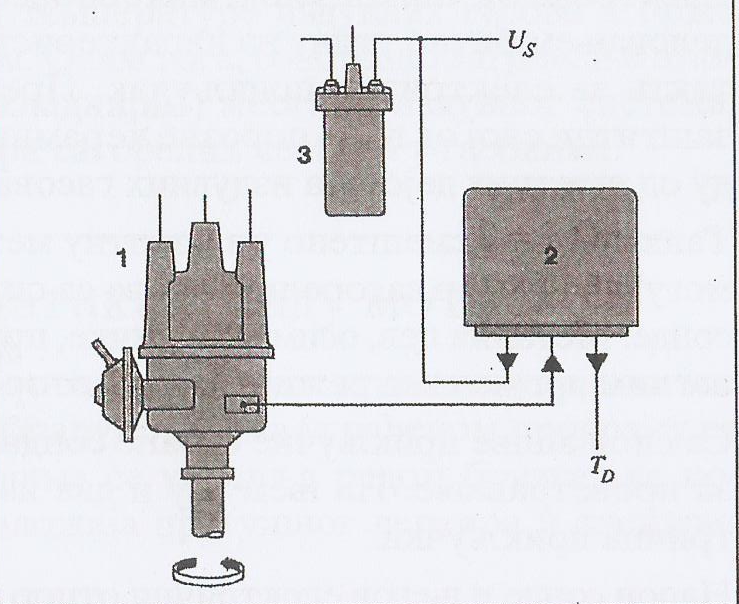
\includegraphics[width=0.5\textwidth]{slike/5.png}
    \caption{Мерење броја обртаја}
    \label{fig:mono-sema}
\end{figure}

\section{Температура мотора}

Сензор температуре мотора је NTC отпорник, смештен у месингану чауру са
навојем, у облику сонде. Уграђује се тако да му врх буде потопљен
у расхладну течност. Отпор му опада са порастом температуре.

\begin{figure}[H]
    \centering
    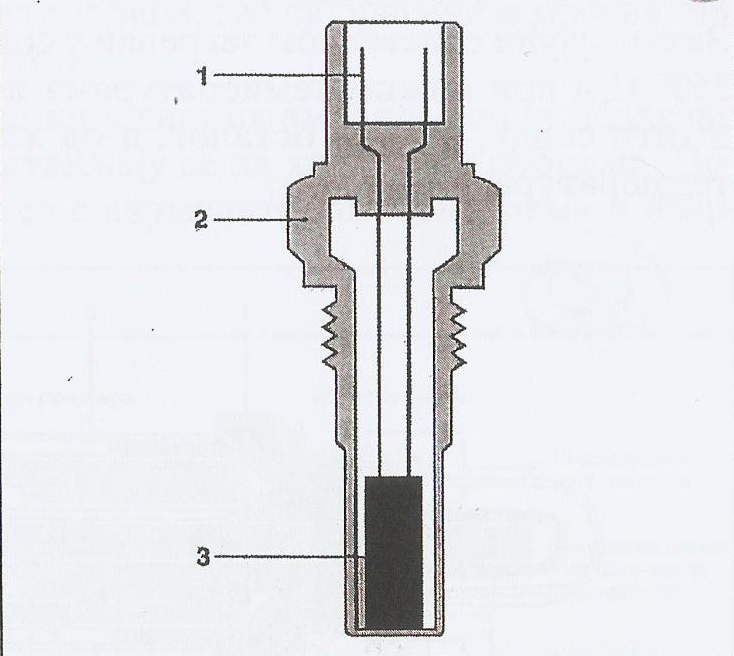
\includegraphics[width=0.5\textwidth]{slike/6.png}
    \caption{Сензор температуре}
    \label{fig:mono-sema}
\end{figure}

\section{Температура усисаног ваздуха}

Густина ваздуха зависи од његове температуре, па се она мора пратити да би се
тачно израчунала количина ваздуха. Сензор је NTC (температурно зависни) отпорник, постављен директно
у ваздушну струју на улазу уређаја за убризгавање, без заштитне чауре, да би
брзо реаговао на промене.

\begin{figure}[H]
    \centering
    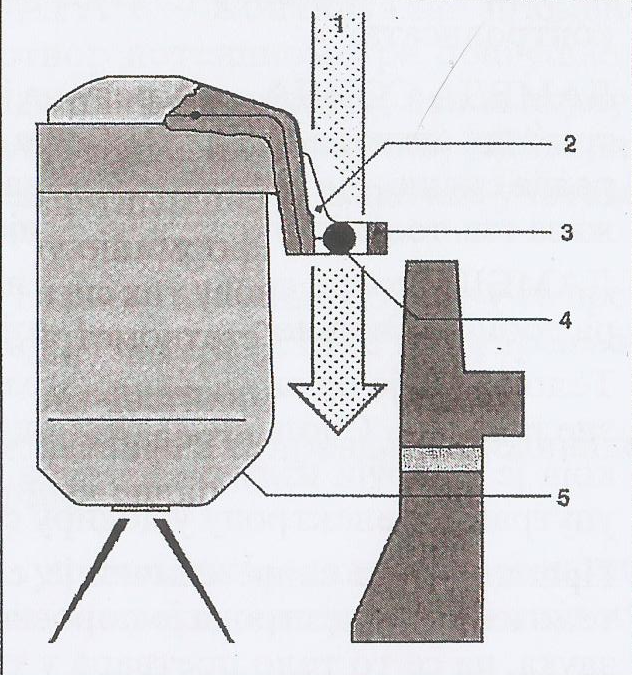
\includegraphics[width=0.5\textwidth]{slike/7.png}
    \caption{Сензор температуре усисаног ваздуха}
    \label{fig:mono-sema}
\end{figure}

\section{Режими рада мотора}

Управљачка јединица добија податке о свим режимима, од празног хода до пуног
оптерећења и кочења мотором, и према њима прилагођава количину горива.
Податак о празном ходу даје \textbf{прекидач празног хода} на корачном мотору:
контакти се затворе када полуга лептира належе на осовину
корачног мотора. Пуно оптерећење јединица препознаје из сигнала
потенциометра лептира.

\begin{figure}[H]
    \centering
    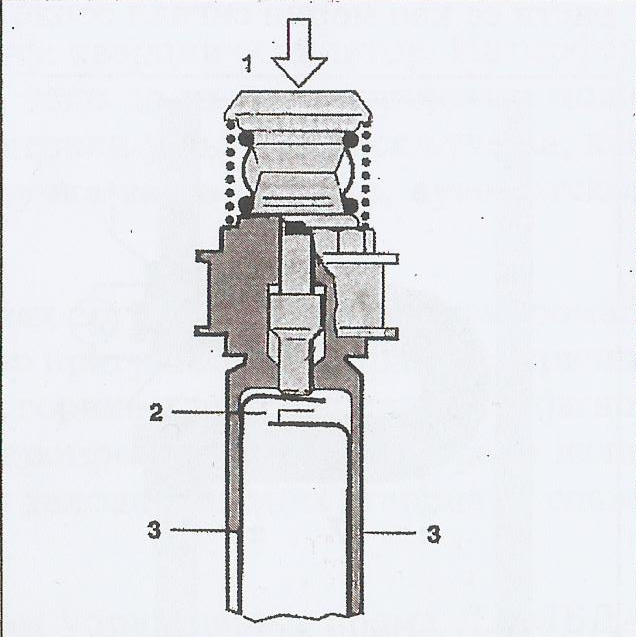
\includegraphics[width=0.5\textwidth]{slike/8.png}
    \caption{Прекидач праног хода}
    \label{fig:mono-sema}
\end{figure}

\section{Напон акумулатора}

Време реаговања бризгаљке зависи од напона акумулатора: при нижем напону она
се спорије отвара. Када напон опадне (на пример при хладном старту), пумпа не
може да одржи пун притисак. Зато управљачка јединица стално прати напон,
који добија директно преко везе са акумулатором, и коригује време
убризгавања.

\section{Састав смеше - ЛАМБДА сонда}

Код возила са ЛАМБДА регулацијом састав смеше мора се строго контролисати.

\begin{kljucno}
      \textbf{ЛАМБДА сонда} поставља се у издувну цев, у струју издувних гасова, и
помоћу електричних сигнала обавештава јединицу о тренутном саставу смеше. Сонда
мора бити довољно загрејана да би радила, и то јој обезбеђује топлота
издувних гасова.
\end{kljucno}

\begin{kljucno}
      \textbf{Принцип рада.} Тело сонде је од керамике, са обе стране обложене
порозним слојем платине (електроде). Спољашња електрода је у додиру са
издувним гасовима, а унутрашња са спољашњим ваздухом. На
вишим температурама керамика постаје проводна за јоне кисеоника. Ако се
садржај кисеоника са две стране разликује, између електрода се јавља напон.
При стехиометријској смеши ($\lambda = 1$) напон сонде нагло скаче:
богата смеша даје напон од око 800~mV, а сиромашна око 200~mV и мање. Тај скок
служи као мерни сигнал.
\end{kljucno}



\begin{figure}[H]
    \centering
    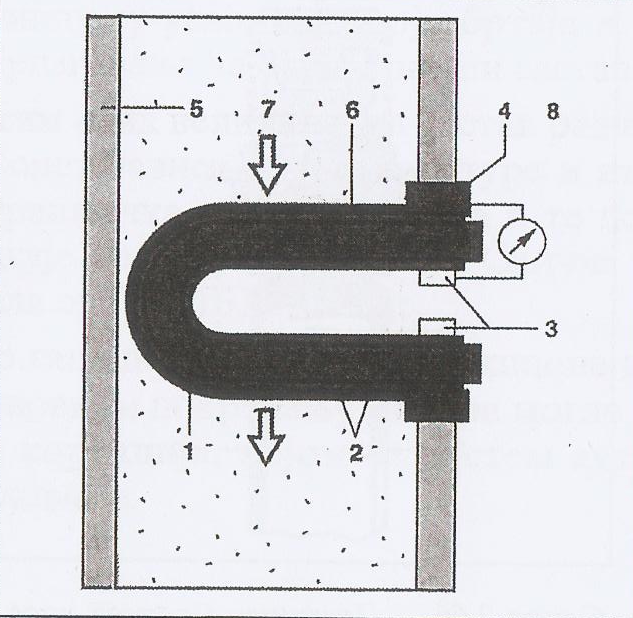
\includegraphics[width=0.5\textwidth]{slike/9.png}
    \caption{ЛАМБДА сонда}
    \label{fig:mono-sema}
\end{figure}


\textbf{Конструкција.} Керамичко тело смештено је у металну чауру са навојем
и електричним прикључцима. Спољна страна је заштићена перфорираном цеви,
која пропушта гасове, а штити сонду од удара честица.

\begin{figure}[H]
    \centering
    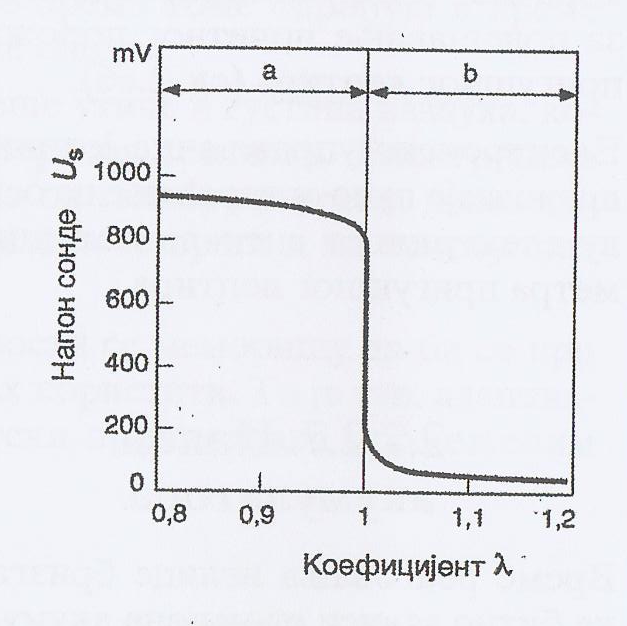
\includegraphics[width=0.5\textwidth]{slike/10.png}
    \caption{Мерење ЛАМБДА сонде}
    \label{fig:mono-sema}
\end{figure}

\textbf{ЛАМБДА сонда са електричним загревањем.} Обична сонда почиње да ради
тек на температури гасова изнад 350\,$^\circ$C. Сонда са сопственим
електричним грејачем у керамичком телу ради већ изнад
200\,$^\circ$C, па регулација почиње брже после хладног старта, а сонда може
да се постави даље од мотора, где је мање оптерећена.

\begin{figure}[H]
    \centering
    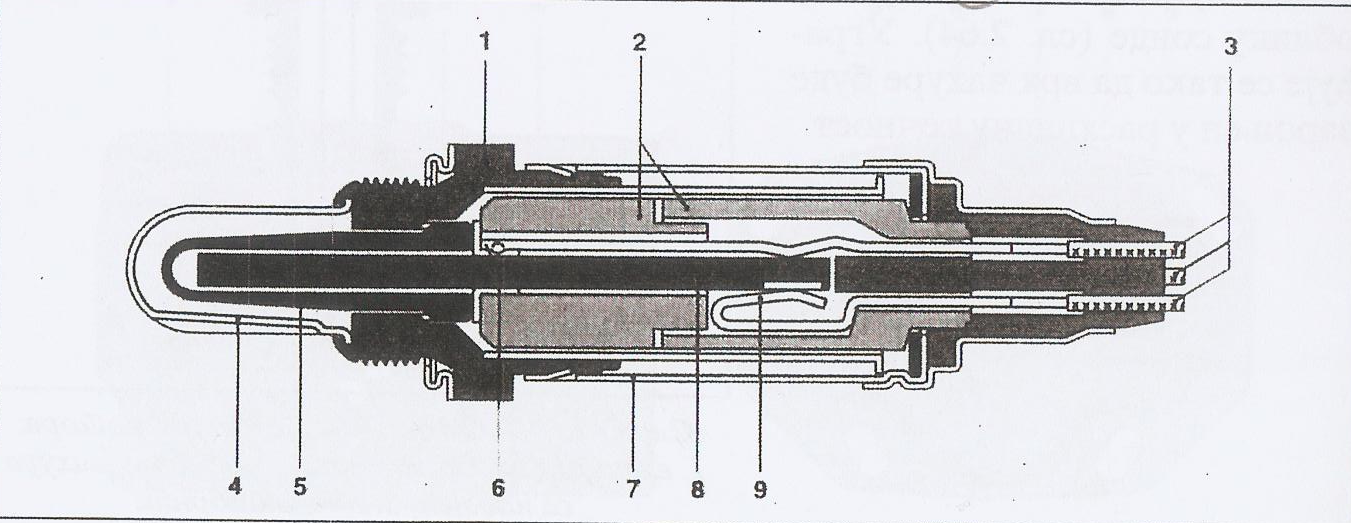
\includegraphics[width=0.5\textwidth]{slike/11.png}
    \caption{ЛАМБДА сонда}
    \label{fig:mono-sema}
\end{figure}

\chapter{Обрада података у управљачкој јединици}

\section{Електронска управљачка јединица}

Кућиште управљачке јединице је од полиамида, ојачаног стакленим влакнима, да би
електронски елементи били заштићени од механичких и термичких утицаја. Јединица
се најчешће смешта у путнички простор или у ниши испод ветробрана, где су мање
вибрације и температуре, а ретко у моторни простор.

Цела електроника налази се на једној штампаној плочи. Излазни степени и
стабилизатор напона постављени су на хладњак са ребрима. Јединица се преко
вишеполног утикача (25 полова) повезује са акумулатором, сензорима и
извршним органима.

\begin{figure}[H]
    \centering
    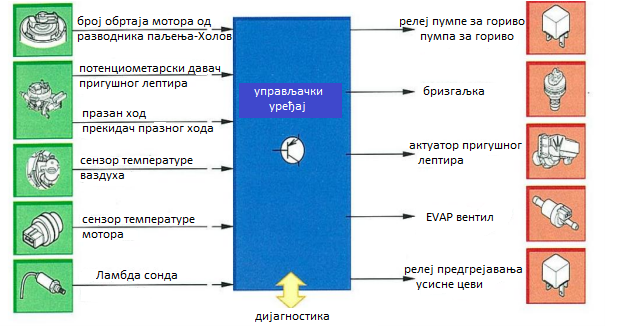
\includegraphics[width=0.7\textwidth]{slike/image1.png}
    \caption{Блок шема система}
    \label{fig:mono-sema}
\end{figure}

\begin{figure}[H]
    \centering
    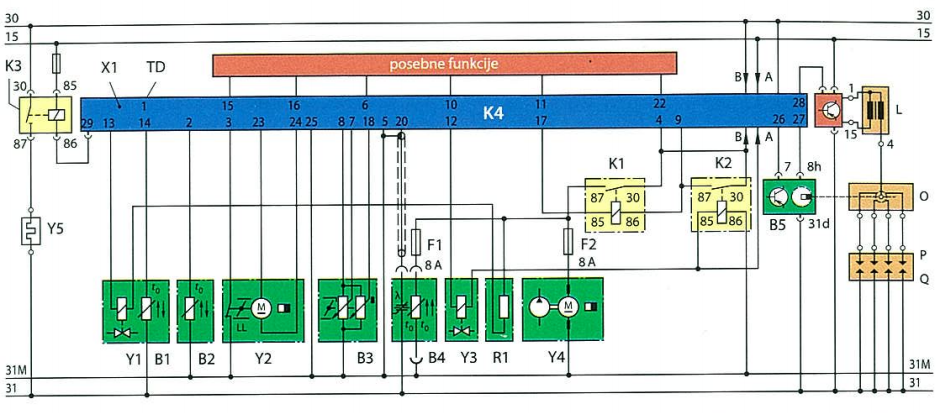
\includegraphics[width=0.9\textwidth]{slike/image2.png}
    \caption{Електрична шема система}
    \label{fig:mono-sema}
\end{figure}

\begin{itemize}[leftmargin=1.6cm, labelwidth=0.7 cm, labelsep=0.3cm, align=left, itemsep=0pt]
    \item[\textbf{В1}] сензор температуре ваздуха
    \item[\textbf{В2}] сензор температуре мотора
    \item[\textbf{В3}] потенциометар пригушног лептира
    \item[\textbf{В4}] ламбда сонда
    \item[\textbf{В5}] Холов сензор
    \item[\textbf{F1, F2}] осигурачи
    \item[\textbf{К1}] релеј пумпе горива
    \item[\textbf{К2}] главни релеј
    \item[\textbf{К3}] релеј за предгрејање усисног ваздуха
    \item[\textbf{К4}] управљачки уређај
    \item[\textbf{R1}] предотпорник
    \item[\textbf{Y1}] централна бризгаљка
    \item[\textbf{Y2}] регулатор пригушног лептира са прекидачем празног хода
    \item[\textbf{Y3}] EVAP вентил
    \item[\textbf{Y4}] пумпа за гориво
    \item[\textbf{Y5}] грејач усисног ваздуха
\end{itemize}

\begin{kljucno}
      \begin{itemize}
    \item Маса јединице изведена је преко два извода. Електронски део за пријем
          сигнала NTC отпорника, ЛАМБДА сонде и потенциометра има посебан спој
          са масом, а друга маса служи за извршне органе, кроз које теку веће
          струје.
    \item Веза са ЛАМБДА сондом изведена је оклопљеним (ширмованим) каблом,
          да би се избегле индуктивне сметње од других струјних кола.
    \item Пумпа за гориво напаја се преко посебног релеја, којим управља
          јединица. По укључењу контакт-кључа пумпа ради неколико секунди, да
          подигне притисак у систему (динамичко управљање пумпом). Ако мотор
          престане да ради, а контакт је и даље укључен (на пример после
          незгоде), релеј аутоматски прекида напајање пумпе.
\end{itemize}
\end{kljucno}

\section{Обрада података}

\begin{figure}[H]
    \centering
    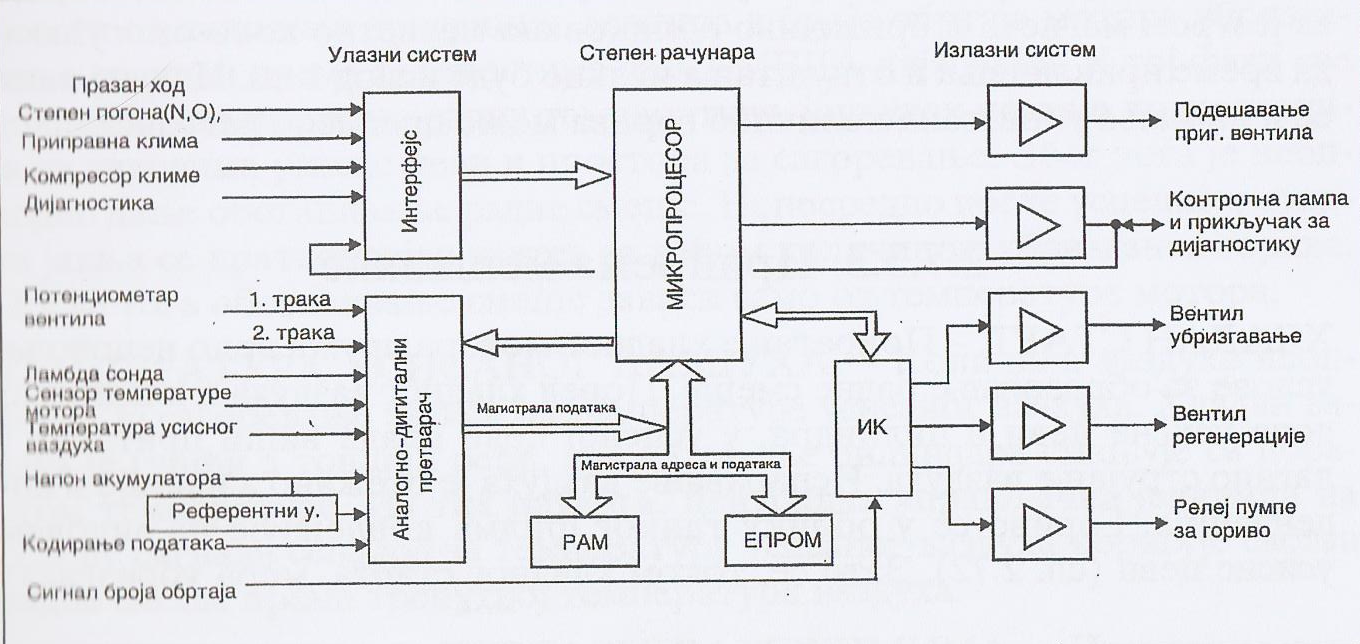
\includegraphics[width=0.7\textwidth]{slike/12.png}
    \caption{Електрична шема ЕУЈ}
    \label{fig:mono-sema}
\end{figure}

\begin{kljucno}
      Прикупљени подаци доводе се до управљачке јединице, која их прилагођава и
обрађује. Према уграђеном програму јединица израђује управљачке сигнале за
бризгаљку, корачни мотор лептира и EVAP вентил.
\end{kljucno}

\begin{kljucno}
      \begin{itemize}
    \item \textbf{Аналогно-дигитални претварач.} Аналогни сигнали (отпор
          потенциометра, напон ЛАМБДА сонде, напон давача температуре, напон
          акумулатора) претварају се у дигиталне, које микропроцесор може да
          обради. Сигнали броја обртаја из система паљења већ су импулси, па
          се обликују посебним колом.
    \item \textbf{Микропроцесор} прима податке од сензора преко интерфејса и
          А/Д претварача и, према програму, израчунава време убризгавања.
          Повезан је са меморијом \textbf{EPROM}, у којој су програм и
          подаци (кодови, дијаграми), и са меморијом \textbf{RAM}, у коју се
          уписују адаптивне корекције. Да се подаци не би изгубили после
          гашења мотора, RAM је стално повезан са акумулатором. Радну
          учестаност од 6~MHz даје кварцни осцилатор.
    \item \textbf{Излазни степени} су појачавачи са транзисторима снаге, преко
          којих микропроцесор управља бризгаљком, корачним мотором, EVAP
          вентилом, релејем пумпе и контролном лампицом.
\end{itemize}
\end{kljucno}

\section{ЛАМБДА дијаграм}

Основно време убризгавања јединица узима из \textbf{ЛАМБДА дијаграма}, који је
у меморији у облику мапе од 225 радних тачака: за 15 различитих вредности
угла лептира и 15 вредности броја обртаја. За сваку радну тачку
записано је време убризгавања при коме је $\lambda \approx 1$. Подела
дијаграма није линеарна: тачке су гушће при малом оптерећењу и малом броју
обртаја, где су промене највеће.

\begin{figure}[H]
    \centering
    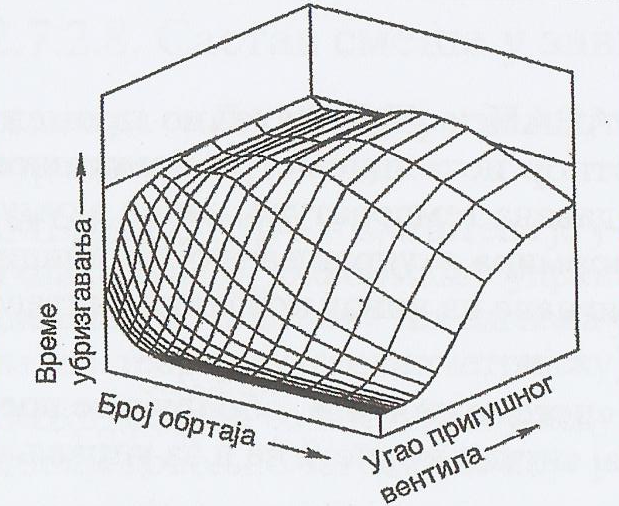
\includegraphics[width=0.5\textwidth]{slike/13.png}
    \caption{ЛАМБДА дијаграм}
    \label{fig:mono-sema}
\end{figure}

Дијаграм важи за загрејан мотор. У осталим условима (хладан мотор, промене
оптерећења) јединица врши корекције, а одступања која утврди ЛАМБДА сонда
памти и користи у даљем раду. То је тзв. адаптивна регулација.


%##################################################################
\chapter{Прилагођавање раду мотора}
%##################################################################

\section{Убризгавање горива}

Задатак система је да радну смешу равномерно распореди на све цилиндре. То
највише зависи од облика усисног колектора, начина и места уградње бризгаљке
и квалитета припреме смеше. Положај бризгаљке код Mono-Jetronic система
одређен је тако да није потребно прилагођавање за поједине типове мотора.

Бризгаљка убризгава гориво у простор изнад пригушног лептира, у купастом
млазу. Ваздух у пролазу поред лептира има највећу брзину и
понесе ситне капљице горива. Део горива ипак падне на зидове колектора и
ствара \textbf{филм горива}, који споро путује ка цилиндрима.

Импулси убризгавања прате импулсе паљења, па се гориво убризгава при сваком
паљењу. Количина горива зависи само од трајања импулса, јер је притисак
сталан.

\section{Хладан старт}

Покретање хладног мотора пружа врло неповољне услове: хладан ваздух, хладни
зидови и низак број обртаја. Гориво слабо испарава и кондензује се на зидовима
усисне цеви и цилиндара. Зато се при хладном старту мора убризгати знатно више
горива него што би одговарало количини ваздуха. Ова кондензација зависи и од
брзине струјања ваздуха: што је она већа, мање горива остаје на зидовима.
Зато се, са порастом броја обртаја, обогаћивање смањује.

Брз и кратак старт тражи да се филм горива брзо створи, а затим да се
обогаћивање брзо смањи, да мотор не би био „поплављен”. Зато се време
убризгавања на почетку старта продужава, а затим скраћује у функцији времена
и броја обртаја.

\begin{figure}[H]
    \centering
    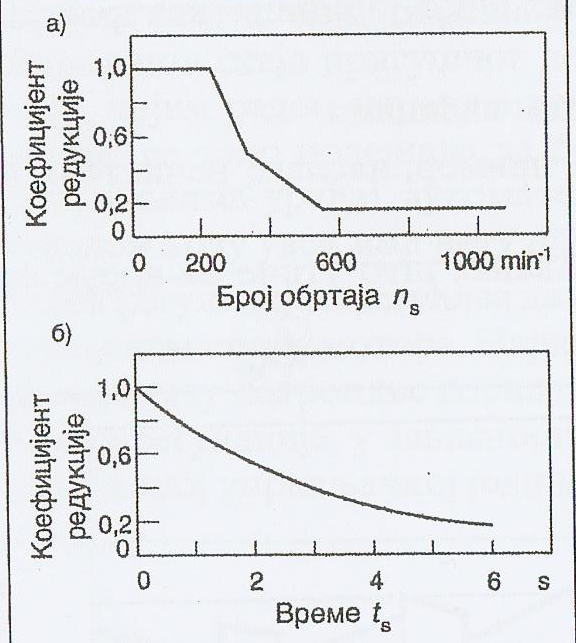
\includegraphics[width=0.4\textwidth]{slike/14.png}
    \caption{График за хладан старт}
    \label{fig:mono-sema}
\end{figure}

\section{Загревање мотора}

У фази загревања, одмах после старта, смеша се обогаћује у зависности од
положаја лептира и броја обртаја, према ЛАМБДА дијаграму. Све док мотор не
достигне радну температуру, гориво се кондензује на хладним зидовима, па је
потребно додатно обогаћивање. Непосредно после старта то је краткотрајан
захтев, а касније обогаћивање зависи само од температуре мотора.

\section{Температура усисаног ваздуха}

Количина ваздуха потребна за сагоревање зависи од његове густине. Хладан
ваздух је гушћи, па се цилиндри пуне већом масом ваздуха. Зато јединица, на
основу сигнала сензора температуре усисаног ваздуха, коригује време
убризгавања.

\section{Празан ход}

Подешавање броја обртаја у празном ходу омогућава стабилан рад мотора са
малим бројем обртаја, што се не мења током целог века мотора. Mono-Jetronic
нема заобилазни вод за ваздух ни биметални вентил. Број обртаја подешава се
\textbf{помоћу корачног мотора}, који мења почетни положај лептира, а тиме и
количину ваздуха. Тако се, без обзира на додатна оптерећења (клима-уређај,
аутоматски мењач, серво-волан итд.), у празном ходу увек одржава прописан број
обртаја. То омогућава да се број обртаја у празном ходу смањи, што смањује
потрошњу горива и штетне материје у издувним гасовима.

Жељени број обртаја зависи од температуре мотора и меморисан је у јединици. Код возила са аутоматским мењачем, када је мењач у положају за
вожњу (D), број обртаја у празном ходу се смањује, да возило не би кренуло
само (крива 1). Када се укључи клима-уређај, број обртаја се повећава
(крива 3), а када се искључи, поново смањује.

\textbf{Регулатор броја обртаја} (у управљачкој јединици) из разлике стварног
и задатог броја обртаја израчунава потребну корекцију положаја лептира.
Лептир се затвара на осовину корачног мотора, а прекидач празног хода
јавља да је лептир у положају празног хода. Јединица тада покреће корачни
мотор док се стварни положај лептира, који региструје потенциометар, не
поклопи са израчунатим.

У јединици су меморисане и вредности почетног положаја лептира у
зависности од температуре мотора, за аутоматски (1) и ручни мењач (2). Ове
вредности рачунар коригује према условима рада (клима-уређај, серво-волан,
стање мотора). Исто подешавање лептира користи се и за ограничење вакуума
током кочења мотором: лептир се отвори мало више, па мотор
добије минималну количину ваздуха потребну за потпуно сагоревање, а ефекат
кочења се мало смањи.

\begin{figure}[H]
    \centering
    \begin{subfigure}[b]{0.32\linewidth}
        \centering
        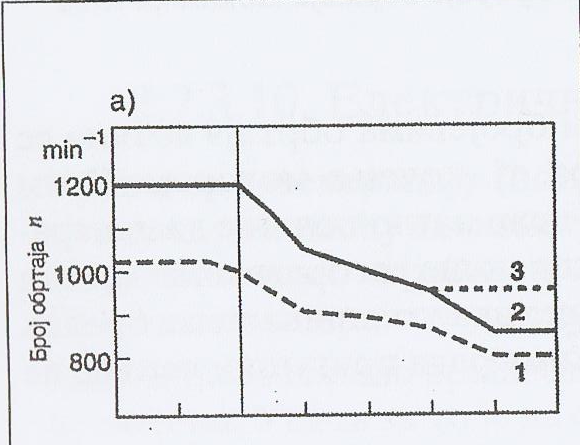
\includegraphics[width=\linewidth]{slike/17.1.png}
        \caption{}
        \label{fig:slika1}
    \end{subfigure}\hfill
    \begin{subfigure}[b]{0.32\linewidth}
        \centering
        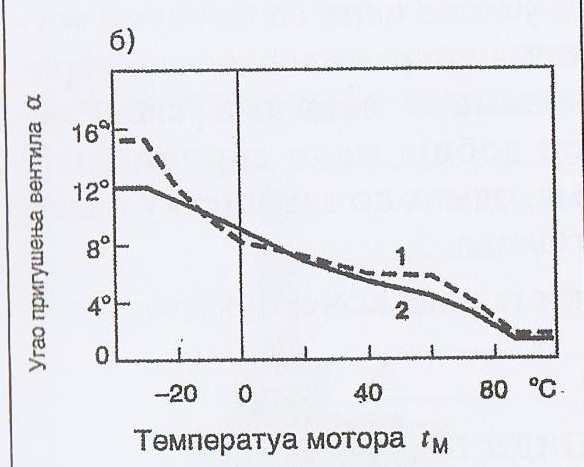
\includegraphics[width=\linewidth]{slike/17.2.png}
        \caption{}
        \label{fig:slika2}
    \end{subfigure}\hfill
    \begin{subfigure}[b]{0.32\linewidth}
        \centering
        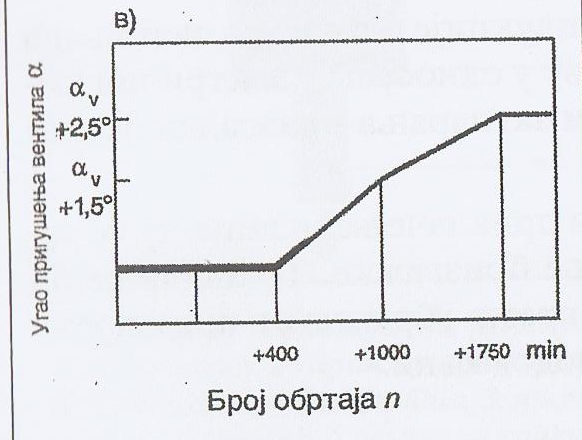
\includegraphics[width=\linewidth]{slike/17.3.png}
        \caption{}
        \label{fig:slika3}
    \end{subfigure}
    \caption{}
    \label{fig:tri_slike}
\end{figure}

\section{Пуно оптерећење}

Када возач потпуно притисне педалу гаса, мотор треба да развије највећу
снагу, за шта је потребна смеша 10--15\,\% богатија од теоријске. Програм
обогаћивања почиње да делује када лептир пређе око 70\,\% највећег отклона,
што јединица препознаје из сигнала потенциометра. ЛАМБДА регулација у том
режиму не делује.

\section{Ограничење броја обртаја}

Прекорачење највећег дозвољеног броја обртаја може изазвати тешка оштећења
мотора. Када број обртаја пређе задату вредност ($n_0$), јединица прекида
импулсе убризгавања, а чим он опадне испод те вредности, убризгавање се
наставља. Наизменичним укључивањем и искључивањем убризгавања број обртаја
се одржава у уском опсегу око највеће дозвољене вредности.

\begin{figure}[H]
    \centering
    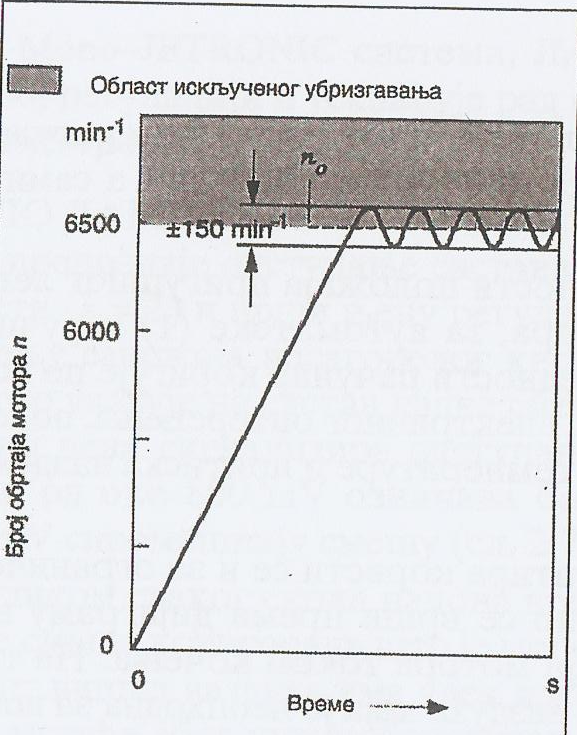
\includegraphics[width=0.4\textwidth]{slike/19.png}
    \caption{Ограничење броја обртаја}
    \label{fig:mono-sema}
\end{figure}

\section{Кочење мотором}

Када возач током вожње подигне ногу са папучице гаса, лептир се потпуно
затвори, а мотор се преко точкова и даље окреће, тј. кочи возило. Тај режим се
зове \textbf{кочење мотором}. Ради уштеде горива и бољег квалитета издувних
гасова, јединица тада прекида убризгавање (функција CAT OFF).

Ако број обртаја у том режиму пређе одређену вредност (праг бр. 2), а лептир је затворен, убризгавање се прекида и мотор остаје без
горива. Када број обртаја опадне испод одређене вредности (око
1200~min$^{-1}$, праг бр. 3), убризгавање се поново укључује. Ако број обртаја
нагло опада (на пример када возач притисне квачило), убризгавање се укључује
и раније (праг бр. 1). Тако се спречава да мотор падне испод празног хода и
угаси се.

При поновном укључењу убризгавања мора се узети у обзир да је, током кочења,
филм горива на зидовима усисне цеви испарио, јер је у цеви био велики
потпритисак. Да би се филм поново створио и мотор не би добио сиромашну
смешу, одмах по завршетку режима кочења додаје се један додатни импулс
убризгавања, чије трајање зависи од трајања режима кочења.

\section{Принудна вожња у случају квара}

Управљачка јединица функцијом \textbf{самодијагностике} непрекидно контролише
исправност и веродостојност сигнала свих сензора. Ако неки сензор даје
сигнале изван програмираних граница, или ако је прекинута веза, јединица
то региструје као квар.

Систем је програмиран тако да возило и у случају квара не остане у квару:
омогућена је \textbf{принудна вожња} до сервиса. Јединица тада, уместо
неисправног сигнала, користи програмирану замену:

\begin{itemize}[noitemsep]
    \item ако откаже сензор температуре, користи се резервна вредност (на
          пример 20\,$^\circ$C за усисни ваздух и 100\,$^\circ$C за мотор),
    \item ако откаже ЛАМБДА сонда, регулација се искључује, а време
          убризгавања израчунава се само према меморисаним вредностима,
    \item ако се изгуби сигнал потенциометра лептира, губи се један од главних
          података за израчунавање времена убризгавања. Тада јединица
          убризгава гориво са две фиксне дужине импулса, које се мењају
          зависно од броја обртаја, а корачни мотор поставља лептир у положај
          за празан ход.
\end{itemize}

Јединица памти откривене грешке у меморији. Прикључивањем уређаја за
дијагностику меморија грешака се очитава, што знатно олакшава откривање
кварова.

\section{Компензација у прелазним режимима}

При промени оптерећења, када се лептир нагло помери, јединица врши
\textbf{динамичку корекцију} састава смеше. Код централног убризгавања она је
сложенија него код убризгавања у више тачака, јер се гориво, пре него што
стигне до цилиндара, делом таложи на зидовима и тек онда испарава.

У празном ходу и делимичном оптерећењу у усисној цеви је низак притисак, па
гориво лако испарава и филм на зидовима је танак. Када се лептир нагло
отвори, притисак порасте, испаравање се смањује и филм се задебља. Тај део
горива недостаје у цилиндрима, па би мотор „штуцао” на сиромашној смеши.
Обрнуто, када се лептир нагло затвори, филм брзо испари и смеша постаје
пребогата. Јединица то спречава тако што, према брзини промене угла лептира
(сигнал потенциометра), при отварању привремено продужава, а при затварању
скраћује импулсе убризгавања.

\section{ЛАМБДА регулација}

ЛАМБДА регулација одржава коефицијент вишка ваздуха што ближе
стехиометријској вредности ($\lambda = 1$), што је услов за ефикасан рад
трокомпонентног катализатора. Регулација је надређена основној
регулацији и усклађује рад система са функцијом катализатора.

\textbf{Коло ЛАМБДА регулације.} Сонда у издувној цеви прати садржај
кисеоника и јавља јединици да ли је смеша богата (напон изнад око 800~mV) или
сиромашна (испод око 200~mV). При сваком скоку напона јединица мења време
убризгавања у супротном смеру: ако је смеша богата, скраћује импулсе, а ако је
сиромашна, продужава их. Смеша зато стално благо осцилује око
$\lambda = 1$. Регулација само исправља мала одступања од ЛАМБДА дијаграма.

\begin{figure}[H]
    \centering
    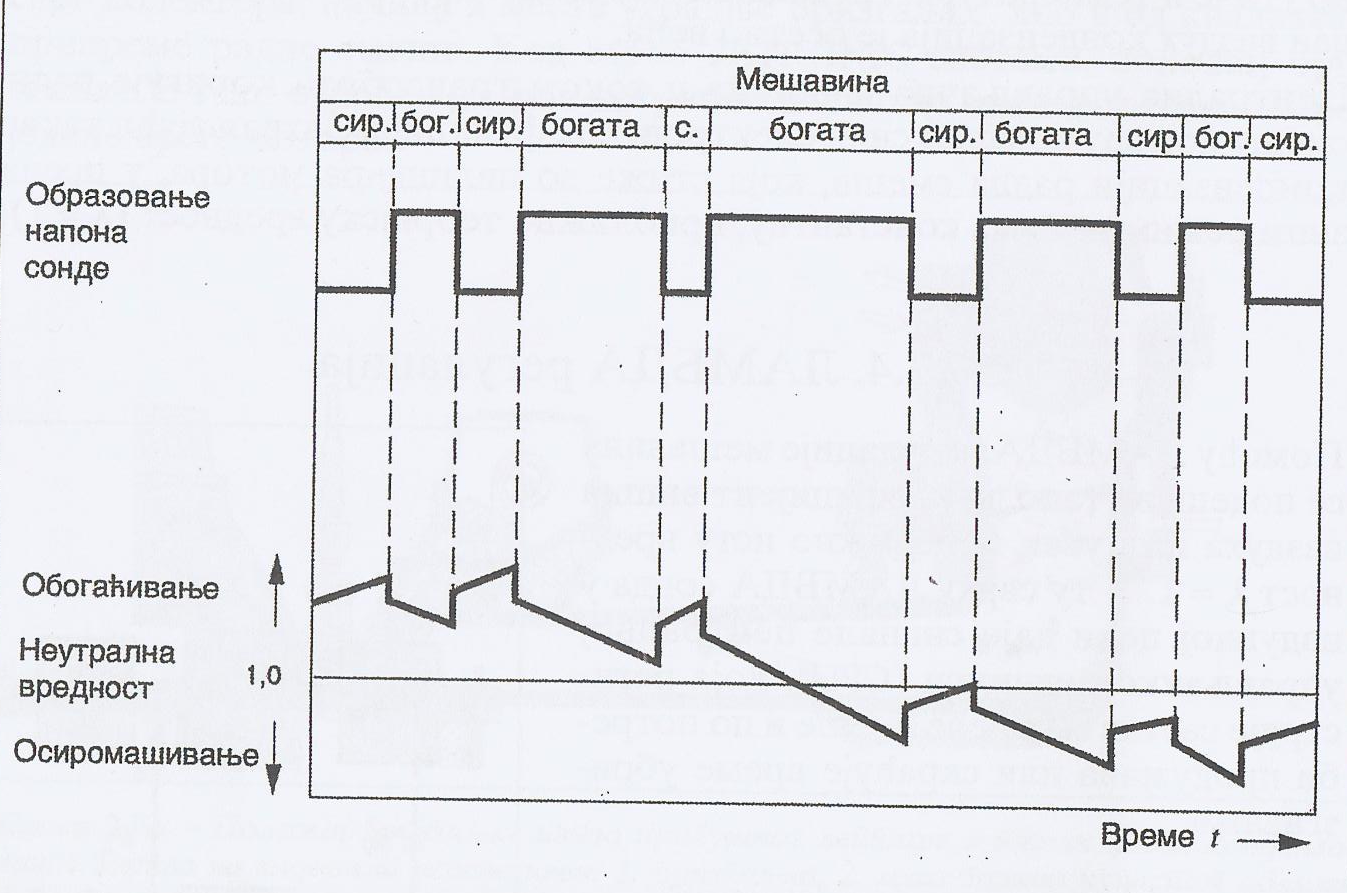
\includegraphics[width=0.5\textwidth]{slike/15.png}
    \caption{ЛАМБДА регулација}
    \label{fig:mono-sema}
\end{figure}

\section{Адаптација радне смеше}

Адаптацијом смеше јединица неутралише сталне неповољне утицаје, као што су:

\begin{itemize}[noitemsep]
    \item промена атмосферског притиска на већим висинама,
    \item непрецизно мерење протока ваздуха, на пример због наслага нечистоће
          на пригушном лептиру,
    \item истрошеност делова уређаја за убризгавање, што утиче на време
          отварања бризгаљке.
\end{itemize}

Атмосферски притисак утиче на целом подручју рада, а грешке у мерењу ваздуха
највише се осећају при малим количинама ваздуха (празан ход), где мала грешка
у углу лептира много мења пуњење. Када се таква грешка јави, ЛАМБДА регулација
је стално исправља у истом смеру. Јединица то препознаје и корекцију
постепено упише у меморију, корак по корак, док коефицијент вишка ваздуха не
буде $\lambda = 1$ и без помоћи регулације. Учесталост ових корака
зависи од оптерећења и броја обртаја мотора.

\begin{figure}[H]
    \centering
    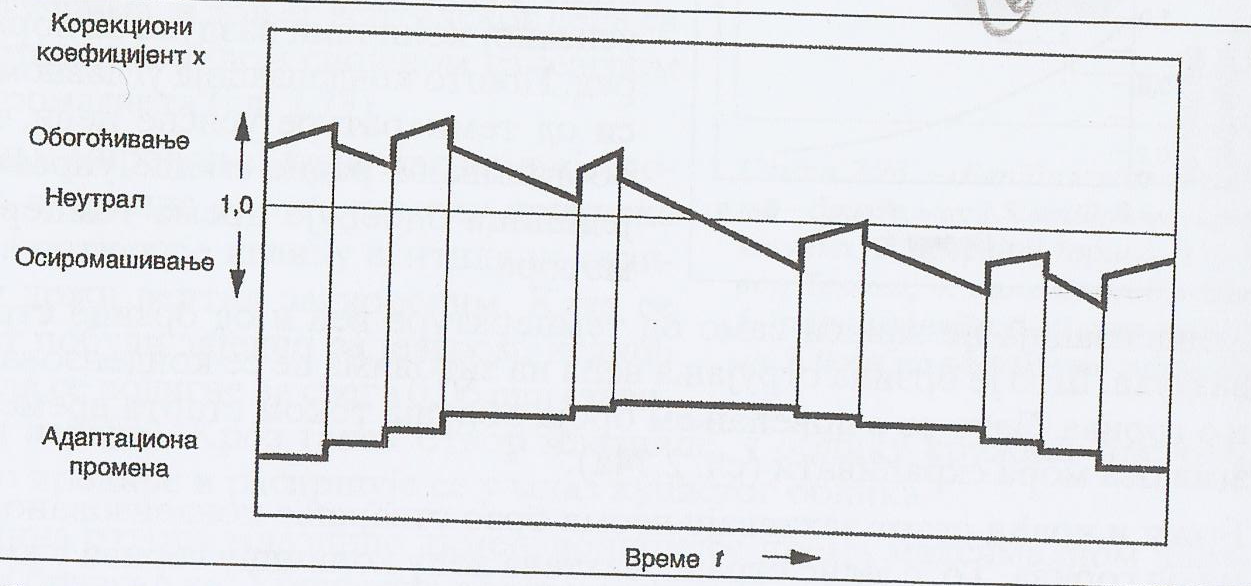
\includegraphics[width=0.5\textwidth]{slike/16.png}
    \caption{Адаптација радне смеше}
    \label{fig:mono-sema}
\end{figure}

\section{Компензација пада напона}

Због самоиндукције намотаја, бризгаљка се отвара са извесним закашњењем у
односу на електрични импулс, а затвара се брже. Средња вредност времена
отварања и затварања износи око 0,8~ms. Напон акумулатора много више утиче на
привлачење игле (отварање) него на отпуштање. Без електронске компензације
то би значило да би, при нижем напону, количина убризганог горива била
недовољна.

\begin{figure}[H]
    \centering
    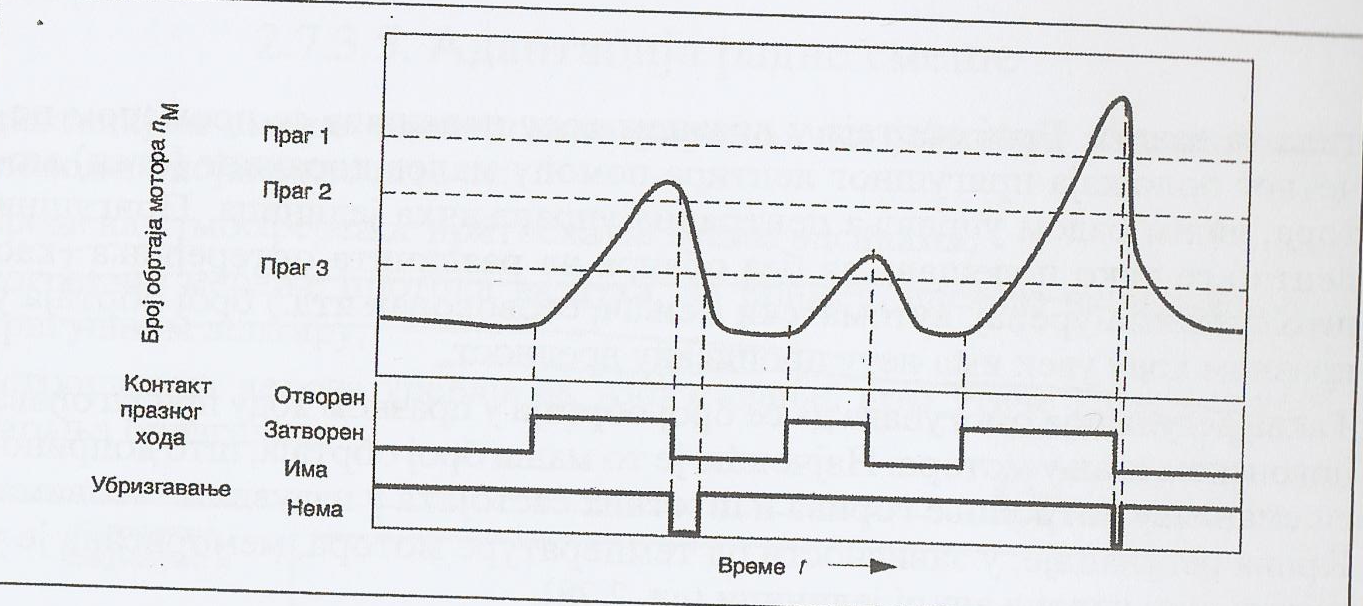
\includegraphics[width=0.5\textwidth]{slike/20.png}
    \caption{Компензација пада напона}
    \label{fig:mono-sema}
\end{figure}

Јединица зато стално прати напон и по потреби продужава импулс убризгавања.
Осим тога, од напона зависи и број обртаја пумпе, па и проток горива. Ако
напон знатно опадне (на пример при хладном старту), пумпа не може да одржи
пун притисак, али и то се компензује продужењем импулса, сразмерно паду
напона. Капацитет пумпе код ових система ипак је довољно велики да
компензација због пада притиска обично није потребна.

\end{document}